% =============================================================================
% retrieval.tex — an explanatory packet for step_7/lib/retrieval.py
%
% The "find me the right page" brain of the Solanus archival tool: contextual
% retrieval, hybrid + RRF + rerank, HyDE / RAG-Fusion, the adaptive router,
% Self-RAG / CRAG, multimodal/ColPali, and RAPTOR — what each is, WHY it helps
% this corpus, and how it is wired (or planned).
%
% Build (keeps ALL aux files in build/):
%     latexmk -pdf -outdir=build retrieval.tex
% so only retrieval.tex and build/retrieval.pdf matter. Nothing exotic required.
% =============================================================================
\documentclass[11pt]{article}
\usepackage{lmodern}
\usepackage[T1]{fontenc}

% --- Packages ---------------------------------------------------------------
\usepackage[margin=1in]{geometry}
\usepackage{amsmath,amssymb}
\usepackage{microtype}
\microtypesetup{expansion=false}
\usepackage{enumitem}
\usepackage{booktabs}
\usepackage{xcolor}
\usepackage{hyperref}
\usepackage{listings}
\usepackage{tikz}
\usepackage[most]{tcolorbox}
\usetikzlibrary{arrows.meta, positioning, shapes.geometric, calc, fit, backgrounds}
\usepackage{placeins}   % \FloatBarrier to keep figures inside their section
\usepackage{caption}
\captionsetup{font=small,skip=8pt}

\hypersetup{colorlinks=true, linkcolor=blue!50!black,
            urlcolor=blue!50!black, citecolor=blue!50!black}

% --- Coloured callout boxes (cf. the example explainers) --------------------
\newtcolorbox{tldrbox}[1][]{
  colback=blue!5, colframe=blue!50!black, fonttitle=\bfseries,
  title={#1}, sharp corners, boxrule=0.6pt}

\newtcolorbox{primerbox}[1][]{
  colback=yellow!10, colframe=orange!70!black, fonttitle=\bfseries,
  title={#1}, sharp corners, boxrule=0.6pt}

\newtcolorbox{caveatbox}[1][]{
  colback=red!4, colframe=red!55!black, fonttitle=\bfseries,
  title={#1}, sharp corners, boxrule=0.6pt}

% --- Listings (Python) ------------------------------------------------------
\definecolor{codebg}{RGB}{248,248,248}
\definecolor{codekw}{RGB}{0,0,180}
\definecolor{codecmt}{RGB}{0,128,0}
\definecolor{codestr}{RGB}{170,55,0}
\lstset{
  basicstyle=\ttfamily\small,
  backgroundcolor=\color{codebg},
  keywordstyle=\color{codekw}\bfseries,
  commentstyle=\color{codecmt}\itshape,
  stringstyle=\color{codestr},
  showstringspaces=false,
  language=Python,
  breaklines=true,
  columns=fullflexible,
  frame=single,
  framesep=4pt,
  rulecolor=\color{black!20},
}

% --- Convenience macros -----------------------------------------------------
\newcommand{\code}[1]{\texttt{#1}}
\newcommand{\file}[1]{\texttt{#1}}

\title{\bfseries Finding the Right Page\\[2pt]
\large An explanatory packet for \texttt{step\_7/lib/retrieval.py}}
\author{Solanus Casey Archival Tool --- step\_7}
\date{}

\begin{document}
\maketitle

\begin{abstract}
This packet walks through the retrieval module --- the part of the archival tool that, given a
question about Father Solanus Casey's letters and notebooks, returns the handful of passages that
answer it, each carrying enough provenance to cite the \emph{exact scanned region}. We build the
idea up from first principles: why lexical and semantic search need each other, how Reciprocal Rank
Fusion marries them, what a reranker adds, how query transforms (HyDE, RAG-Fusion) and an adaptive
router decide how hard to work, and how a Self-RAG/CRAG grader lets an \emph{archive} honestly say
``I could not find this.'' We close with the three frontier techniques the corpus most wants next
--- Contextual Retrieval, multimodal/ColPali, and RAPTOR --- marking carefully what is wired today
versus planned. Wording follows the source comments closely, reorganised into prose.
\end{abstract}

\tableofcontents
\bigskip

% =============================================================================
\section{TL;DR}
% =============================================================================

\begin{tldrbox}[The thirty-second version]
\begin{itemize}[leftmargin=*]
  \item \textbf{The job.} Turn a question into a short, ranked list of passages, each tagged with
        \code{doc\_id} $\to$ \code{rid} $\to$ \code{vertices} so we can draw a box on the original
        scan (an IIIF deep-zoom citation). If the right page never makes the shortlist, no prompt can
        rescue the answer --- retrieval is where accuracy is won or lost.
  \item \textbf{The free path already works.}
        \code{router (heuristic)} $\to$ \code{BM25 + dense} $\to$ \code{RRF} $\to$ \code{grade}.
        No API key, no paid call, no model download. BM25 nails exact names and dates; dense
        embeddings catch paraphrase; RRF fuses them without calibrating their incompatible scores.
  \item \textbf{Every upgrade is a toggle, and every paid toggle is gated.} Rerank, HyDE,
        multi-query/RAG-Fusion, the LLM router, and the per-document grader are all off by default
        and each routes its cost through \file{lib/costlog.py}. You opt into spend; you never trip
        into it.
  \item \textbf{Built for an archive, so it can abstain.} A free Self-RAG/CRAG grader scores the
        retrieved set (rank margin, lexical overlap, OCR confidence) and returns
        \code{answer} / \code{caveat} / \code{abstain}. A confident wrong answer is the worst
        outcome in an archive.
  \item \textbf{The biggest pending win is Contextual Retrieval.} Prepending a one-line context to
        each terse, date-less notebook entry before indexing is what makes ``\,22 --- reports
        cured.\,'' findable at all. It is an \emph{indexing-time} technique (chunk/embed stage), so
        it sits upstream of this file --- and is the recommended next build.
\end{itemize}
\end{tldrbox}

% =============================================================================
\section{Why retrieval is the hard part (and a tiny jargon primer)}
% =============================================================================

A large language model is a brilliant talker with no memory of our archive. Retrieval-Augmented
Generation (RAG) fixes that by \emph{looking things up first}: we find the most relevant passages,
hand them to the model, and ask it to answer \emph{only} from what it was given. So the quality of
the final answer is capped by the quality of retrieval. Everything in \file{lib/retrieval.py} exists
to raise that cap.

\begin{primerbox}[Skip if you already know BM25, embeddings, cosine similarity, and cross-encoders]
\textbf{Sparse / lexical (BM25).} Treats text as a bag of words and scores overlap of the
\emph{actual tokens}. Great at exact strings --- a surname like \emph{O'Donnell}, a date like
\emph{1933}.

\textbf{Dense / semantic (embeddings).} Maps a passage to a vector so that passages with similar
\emph{meaning} sit close together. Great at paraphrase --- it knows \emph{favor}, \emph{miracle},
and \emph{answered prayer} are neighbours.

\textbf{Cosine similarity.} The cosine of the angle between two vectors: $+1$ same direction
(very similar), $0$ unrelated, $-1$ opposite. Our vectors are pre-normalised, so cosine is just a
dot product.

\textbf{Cross-encoder (reranker).} Instead of embedding the query and passage separately, it reads
them \emph{together} and outputs one relevance score. Much sharper, much slower --- so we only ever
run it on a short candidate list.
\end{primerbox}

Our corpus makes this concrete and a little brutal. The letters are reasonably well-formed prose,
but the notebooks are a running register written in shorthand. A real entry looks like:
\begin{quote}\small\itshape
``22 --- reports cured.''
\end{quote}
No year. No surname. No condition. On its own that chunk is almost impossible to retrieve --- and
yet it may be the single record that answers ``which favors were reported cured in 1933?'' Holding
that example in mind explains nearly every design choice below.

% =============================================================================
\section{The data shape that makes citation possible}
% =============================================================================

Everything the module returns is a \code{Hit}: it mirrors the chunk shape from \file{lib/chunks.py}
(\code{id} / \code{kind} / \code{text} / \code{meta}) and adds a fused \code{score}, a
\code{provenance} dict, and a \code{components} debug dict (which retriever ranked it where). The
\code{provenance} is the reason this is an \emph{archival} tool and not a chatbot:

\begin{itemize}[leftmargin=*]
  \item For a \textbf{notebook entry}, the chunk's \code{meta.rid} points at one region. We look that
        region up in \code{\_region\_index()} --- a one-time map of
        \code{"doc\_id::rid" $\to$ \{vertices, min\_conf, \dots\}} read from the same step\_6 JSON
        the chunker reads --- and the citation reaches the \emph{exact box} on the page.
  \item For a \textbf{letter} (several regions joined into one chunk) there is no single \code{rid},
        so we record the page-level location and let the UI resolve per-region detail from the
        source record. The citation still always reaches the right page.
\end{itemize}

\noindent The module is, by design, a set of \emph{pure functions returning ranked \code{Hit}s}:
nothing mutates the corpus, nothing writes files. That keeps each piece testable and lets the dev
harness flip any subset on while measuring every model combination.

% =============================================================================
\section{The pipeline at a glance}
% =============================================================================

The adaptive entry point \code{route\_and\_retrieve} wires the whole brain together. A query flows
left to right; the dashed boxes are paid and \emph{off by default}.

\begin{center}
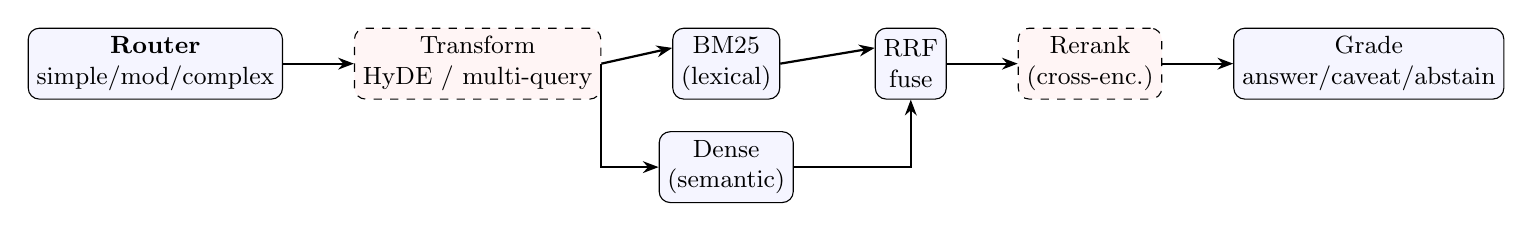
\begin{tikzpicture}[
    node distance=6mm and 9mm,
    box/.style={draw, rounded corners, align=center, minimum height=9mm,
                inner sep=3pt, font=\small, fill=blue!4},
    paid/.style={draw, dashed, rounded corners, align=center, minimum height=9mm,
                 inner sep=3pt, font=\small, fill=red!4},
    arr/.style={-{Stealth[length=2mm]}, thick}]
  \node[box] (route)  {\textbf{Router}\\simple/mod/complex};
  \node[paid, right=of route] (xform) {Transform\\HyDE / multi-query};
  \node[box, right=of xform] (bm25)   {BM25\\(lexical)};
  \node[box, below=4mm of bm25] (dense){Dense\\(semantic)};
  \node[box, right=12mm of bm25] (rrf) {RRF\\fuse};
  \node[paid, right=of rrf] (rerank)  {Rerank\\(cross-enc.)};
  \node[box, right=of rerank] (grade) {Grade\\answer/caveat/abstain};

  \draw[arr] (route) -- (xform);
  \draw[arr] (xform.east) -- ([yshift=2mm]bm25.west);
  \draw[arr] (xform.east) |- (dense.west);
  \draw[arr] (bm25.east) -- ([yshift=2mm]rrf.west);
  \draw[arr] (dense.east) -| (rrf.south);
  \draw[arr] (rrf) -- (rerank);
  \draw[arr] (rerank) -- (grade);
\end{tikzpicture}
\end{center}

\noindent The \emph{free path} is the solid boxes only:
\code{router} $\to$ \code{BM25 + dense} $\to$ \code{RRF} $\to$ \code{grade}. We now take each stage
in turn.

% =============================================================================
\section{The router: spend brainpower in proportion to the question}
% =============================================================================

\noindent ``When was Solanus born?'' deserves one cheap lookup. ``List every cancer favor reported
in 1933 and how each turned out'' deserves decomposition, several queries, and synthesis. Treating
them identically either wastes money on the easy one or under-serves the hard one.

\code{route\_query} sorts a query into \textbf{simple}, \textbf{moderate}, or \textbf{complex} from
cheap signals: length, question words (\emph{who/when/where}), aggregate markers
(\emph{every/how many/timeline/compare}), and conjunctions that hint at multi-part asks. It returns a
\emph{recommendation}, never a command:

\begin{lstlisting}
{"complexity": "complex",
 "strategy": "decompose -> multi-query retrieval + RRF (+ rerank), then synthesis",
 "reason": "aggregate/multi-part markers or a long, compound question",
 "suggest": {"use_multiquery": True, "multihop": True}}
\end{lstlisting}

\noindent The crucial design point: multi-query is a \emph{paid} LLM call, so the router never spends
on its own. The transform runs only if the caller set \code{use\_multiquery}, \emph{or} if
\code{auto\_apply\_route=True} (the switch by which an agent opts into letting the router escalate).
That is why the default path stays at \textbf{exactly zero paid calls even on a ``complex'' query}.
An LLM classifier (\code{use\_llm\_router}) handles genuinely ambiguous phrasing and \emph{degrades
to the heuristic on any failure}, so the router can never become a hard dependency on the model.
\emph{Why it helps us:} the corpus mixes trivial biographical facts with real aggregate archival
questions; routing keeps the cheap ones cheap and reserves the heavy machinery for the asks that
need it (the literature reports roughly $-28\%$ cost and $+8\%$ accuracy from adaptive routing).

% =============================================================================
\section{Hybrid retrieval: BM25 and dense, because each rescues the other}
% =============================================================================

\subsection{BM25 --- the lexical workhorse}

BM25 scores a passage by summing, over each query term, three intuitions multiplied together:

\[
\text{score}(d) \;=\; \sum_{t \in q} \underbrace{\mathrm{IDF}(t)}_{\text{rare words count more}}
\cdot
\frac{f_{t,d}\,(k_1+1)}
     {f_{t,d} + k_1\!\left(1 - b + b\,\dfrac{|d|}{\overline{|d|}}\right)},
\]

where $f_{t,d}$ is how often term $t$ appears in document $d$. The numerator rewards term frequency;
$k_1$ \emph{saturates} it so the tenth occurrence matters less than the first; $b$ applies
\emph{length normalisation} so a long document does not win merely by being long; and IDF up-weights
rare terms. We keep the standard $k_1{=}1.5$, $b{=}0.75$.

For us BM25 is unbeatable on \emph{exact tokens}: we tokenise keeping apostrophes (so
\emph{O'Donnell} survives) and digits (so \emph{1933} is a real token). We prefer the
\code{rank\_bm25} package but ship a small \emph{correct} \code{BM25Okapi} fallback, so the free path
never depends on an install --- if the package is missing the module quietly uses the fallback.

\subsection{Dense --- the semantic workhorse}

\code{dense\_search} embeds the query in a chosen \emph{space} (\code{model@dim}, e.g.
\code{gemini-embedding-001@1536}) and cosine-searches that vector-store partition. The query is
embedded with \code{task="query"} so providers use their asymmetric query-side encoding. Dense
catches the paraphrase BM25 is blind to.

Crucially, dense \emph{degrades gracefully}. If the partition for that space has not been built, or a
hosted embedder has no API key, \code{retrieve} catches the \code{FileNotFoundError} /
\code{RuntimeError} and falls back to BM25-only rather than crashing the whole retriever. (A genuine
bug like a bad model name still raises \code{ValueError} --- we deliberately do \emph{not} swallow
that.) So the free/offline path always returns \emph{something}.

\subsection{Why both, on our corpus}

The notebook entries are terse and idiosyncratic. Sometimes the only handle is an exact name and
BM25 wins; sometimes it is a concept the writer phrased unusually and dense wins. Running both and
fusing them is strictly safer than betting on either alone --- which is the entire motivation for the
next section.

% =============================================================================
\section{RRF: fusing ranked lists without calibrating their scores}
% =============================================================================

Here is the trap. BM25 scores might run $0$--$15$; cosine similarities run $-1$--$1$. If we simply
\emph{add} them, whichever retriever happens to emit bigger numbers silently dominates the fusion.
\textbf{Reciprocal Rank Fusion} sidesteps this entirely: it throws the raw scores away and uses only
each item's \emph{rank position}.

\[
\mathrm{RRF}(d) \;=\; \sum_{\ell \,\in\, \text{lists}}
\frac{w_\ell}{k + \mathrm{rank}_\ell(d)}.
\]

A passage near the top of \emph{either} list earns a big contribution; the constant $k$ (default
$60$, the published default) damps the very top ranks so no single retriever can unilaterally decide
the winner. The figure shows the shape of $1/(k+\mathrm{rank})$: front-loaded, but never explosive.

\begin{center}
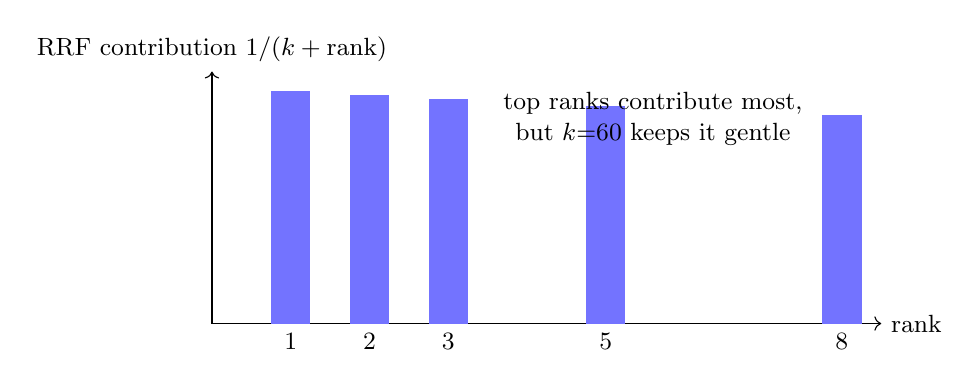
\begin{tikzpicture}[scale=1.0]
  \draw[->] (0,0) -- (8.5,0) node[right] {\small rank};
  \draw[->] (0,0) -- (0,3.2) node[above] {\small RRF contribution $1/(k+\text{rank})$};
  \foreach \r/\lab in {1/1,2/2,3/3,5/5,8/8} {
    \pgfmathsetmacro\h{60/(60+\r)*180}      % exaggerated y-scale for visibility
    \fill[blue!55] (\r-0.25,0) rectangle (\r+0.25, {\h/60});
    \node[below] at (\r,0) {\small \lab};
  }
  \node[align=center, font=\small] at (5.6,2.6)
    {top ranks contribute most,\\ but $k{=}60$ keeps it gentle};
\end{tikzpicture}
\end{center}

\noindent RRF is the project's universal combiner. It fuses BM25 with dense (here), it fuses
\emph{across queries} in RAG-Fusion (\S\ref{sec:transforms}), and it is exactly how a future ColPali
image-retrieval list would be merged with the text retrievers (\S\ref{sec:colpali}) --- one clean,
scale-free operation everywhere.

% =============================================================================
\section{Rerank: the expensive judge that reads query and passage together}
% =============================================================================

First-stage retrieval is cheap and casts a wide net (``give me 50 candidates''). A
\emph{cross-encoder reranker} then re-reads the query \emph{jointly} with each candidate and emits a
single, far sharper relevance score --- the difference between ``these words co-occur'' and ``this
passage actually answers the question.'' Because that joint read is expensive, we feed it only
\code{rerank\_pool} (default $30$) candidates: \emph{retrieve fifty, rerank to a precise few}.

The reranker is the third swappable model axis (\file{lib/providers/rerank.py}), alongside embedding
and generation:
\begin{itemize}[leftmargin=*]
  \item \textbf{local} \code{bge-reranker} via fastembed --- free, offline, runs now;
  \item \textbf{Voyage} \code{rerank-2.5} / \textbf{Cohere} \code{rerank-4-pro} --- real adapters,
        but \emph{paid}: key-gated, and every call is cost-logged.
\end{itemize}
After reranking, the reranker's score becomes the \code{Hit}'s authority and we re-sort; any
candidates beyond the pool keep their fused order behind the reranked ones.

% =============================================================================
\section{Query transforms: HyDE and RAG-Fusion}
\label{sec:transforms}
% =============================================================================

Both transforms are \emph{paid} LLM calls, both default off, both cost-logged inside
\code{llm.generate}.

\subsection{HyDE --- embed a hypothetical \emph{answer}}

A question and its answer are written in different words. ``Who was cured?'' shares almost no
vocabulary with ``Mrs.\ Panyard's cancer was reported cured after enrollment in the Seraphic Mass
Association.'' \textbf{HyDE} (Hypothetical Document Embeddings) asks the LLM to \emph{write} a short,
confident, in-style answer passage and then embeds \emph{that} instead of the question. The fake
answer lives in answer-space, nearer the real passages, so dense recall improves. If the LLM returns
nothing, we fall back to embedding the raw query --- the transform can only help, never break.

\subsection{RAG-Fusion --- many phrasings, one fused result}

Different phrasings surface different true passages: one reader asks about a \emph{favor}, another a
\emph{miracle}, another an \emph{answered prayer}. \code{multi\_queries} asks the LLM for a few
diverse paraphrases (always keeping the original), we retrieve for each, and RRF-fuses the lists --
the same combiner from before, now \emph{across queries}. JSON parsing is forgiving: a malformed
reply simply yields ``no extra variants,'' never a crash.

% =============================================================================
\section{Self-RAG / CRAG: earning the right to answer}
% =============================================================================

In an archive, a confident-but-unsupported answer is the worst possible outcome --- it launders a
guess into something that looks like a citation. So after retrieval we \emph{grade} the result set
before the generator ever sees it.

\subsection{The free grader (\code{grade\_context})}

It uses only signals we already have, so it costs nothing:

\begin{itemize}[leftmargin=*]
  \item \textbf{Top fused score} and the \textbf{margin} between \#1 and \#3 --- a flat distribution
        means the retrieval is ambiguous, with no clear winner.
  \item \textbf{Lexical overlap} between the query terms and the top hits --- did we even match the
        words we were asked about?
  \item \textbf{OCR \code{min\_conf}} on the cited regions --- evidence transcribed at low confidence
        is shaky no matter how well it ranks. This signal is unique to a \emph{scanned} archive and
        we get it for free from the region geometry.
\end{itemize}

\noindent It returns a CRAG-style verdict --- \code{answer} (strong match, adequate overlap),
\code{caveat} (present but shaky: low OCR confidence or flat ranking), or \code{abstain} (top score
or overlap too low) --- plus a blended \emph{confidence} number. The thresholds are deliberately
conservative: for an archive, prefer ``not found'' to a fabrication.

\begin{caveatbox}[Read the confidence number for what it is]
The \code{confidence} returned by \code{grade\_context} is a heuristic blend of overlap, rank margin,
and OCR confidence --- \emph{not} a probability and \emph{not} a correctness guarantee. It is a
guardrail for \emph{when to abstain}, to be tuned against a golden Q\&A set (the evaluation work in
the research plan, Part~E).
\end{caveatbox}

\subsection{The gated per-document grader (\code{grade\_document})}

This is the Self-RAG ``ISREL'' idea: hand the LLM one $(\text{query}, \text{passage})$ pair and get
back a relevance label, used to \emph{filter} a reranked set before generation. It is paid and off by
default. If the judge call fails, it \emph{keeps} the document (labelled \code{partial}) and lets a
human decide --- a grader must never silently drop evidence.

% =============================================================================
\section{Putting it together: \texttt{route\_and\_retrieve}}
% =============================================================================

The adaptive entry point runs the brain the way the agent would:
\begin{enumerate}[leftmargin=*]
  \item \textbf{Route} (free heuristic unless \code{use\_llm\_router}); the route may \emph{suggest}
        multi-query, honoured only if the caller enabled it or set \code{auto\_apply\_route}.
  \item \textbf{Transform}: HyDE \emph{or} multi-query, if enabled/escalated.
  \item \textbf{Retrieve} per query via \code{retrieve} (itself BM25 $+$ dense $+$ RRF $+$ optional
        rerank), then RRF-fuse \emph{across} queries (RAG-Fusion), optionally reranking the fusion.
  \item \textbf{Grade} the final set so the generator knows whether to answer, caveat, or abstain.
\end{enumerate}
It returns a complete, serialisable result --- \code{\{query, route, queries\_used, hits, grade\}} ---
and with default config the \emph{entire function makes zero paid calls}. Each model touchpoint is
individually gated and logged.

\begin{lstlisting}
from lib.retrieval import RetrievalConfig, route_and_retrieve

res = route_and_retrieve("What favors were reported for cancer?")   # FREE
print(res["grade"]["verdict"], res["grade"]["confidence"])          # answer/caveat/abstain
for h in res["hits"]:
    p = h["provenance"]
    print(h["score"], h["kind"], p["doc_id"], "rid=", p["rid"], "pg=", p["page"])
\end{lstlisting}

% =============================================================================
\section{The frontier: three techniques this corpus wants next}
% =============================================================================

The following are documented here and ranked by leverage in \file{RESEARCH\_PLAN.md} (Part~D), but
are \emph{not} yet coded in \file{retrieval.py} --- they are either upstream (indexing-time) or heavy
(a GPU model / an offline LLM build), and are intentionally deferred with clear TODOs. This section
is explicit about wired-versus-planned so nobody assumes a toggle exists that does not.

\subsection{Contextual Retrieval --- the biggest win, sitting \emph{upstream} of this file}

Anthropic's Contextual Retrieval reports a \textbf{$-67\%$ reduction in retrieval failures} from one
move: prepend a 2--3 sentence, LLM-generated context to \emph{each chunk} \emph{before} embedding it
\emph{and} before BM25 indexing. Our notebooks are precisely the case it fixes. Recall the real
entry:
\begin{center}
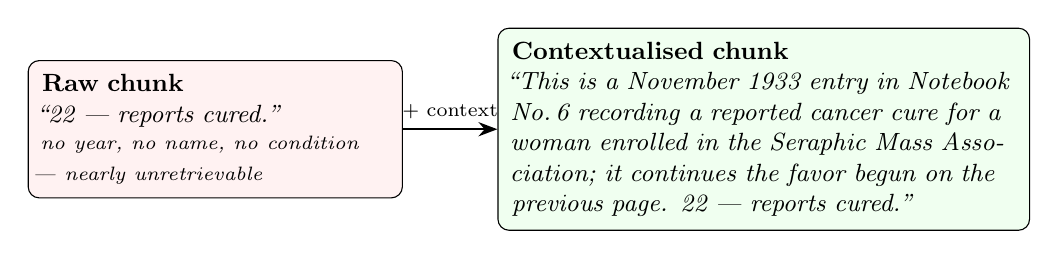
\begin{tikzpicture}[font=\small, node distance=4mm]
  \node[draw, fill=red!5, rounded corners, align=left, text width=4.4cm, inner sep=5pt]
       (raw) {\textbf{Raw chunk}\\\itshape ``22 --- reports cured.''\\[2pt]\scriptsize
              no year, no name, no condition\\ --- nearly unretrievable};
  \node[draw, fill=green!6, rounded corners, align=left, text width=6.4cm, inner sep=5pt,
        right=12mm of raw]
       (ctx) {\textbf{Contextualised chunk}\\\itshape ``This is a November 1933 entry in
              Notebook No.\,6 recording a reported cancer cure for a woman enrolled in the Seraphic
              Mass Association; it continues the favor begun on the previous page. 22 --- reports
              cured.''};
  \draw[-{Stealth[length=2.4mm]}, thick] (raw) -- (ctx)
       node[midway, above, font=\scriptsize] {+ context};
\end{tikzpicture}
\end{center}
Now both BM25 (the literal words \emph{November}, \emph{1933}, \emph{cancer}, \emph{Seraphic}) and
the embedding (the meaning) can find it. Because the context is baked into the \emph{stored} chunk,
this is an \textbf{indexing-time} change: it belongs in the chunk/embed stage, and
\file{retrieval.py} then benefits for free with no code change. It also dovetails with the structural
work in \file{RESEARCH\_PLAN.md} Part~A (cross-page continuation, date reconstruction): those stages
\emph{recover} exactly the date / notebook / continuation context this technique injects.
\textbf{This is the recommended next build.}

\subsection{Multimodal / ColPali --- retrieve over the page \emph{images}}
\label{sec:colpali}

ColPali / ColQwen embed a page \emph{image} as a grid of visual patch vectors and score relevance
with \emph{late interaction} (MaxSim): for each query token, take its best-matching image patch, then
sum those bests. No OCR is involved. On scanned documents, visual recall routinely beats text
(roughly $84\%$ vs $62\%$ in published comparisons) because it sees marginalia, layout, and precisely
the strokes OCR drops. The plan: run ColPali as its \emph{own} retrieval tool over our masked page
PNGs, two-phase (a mean-pooled coarse screen, then MaxSim rerank of the top $\sim 100$), and
\textbf{RRF-fuse} its ranked list with the text retrievers --- the same combiner from before.
\emph{Why for us:} every chunk already carries \code{pdf\_page} provenance, so an image hit cites the
same page; and a handwritten archive is exactly where OCR misses hurt most. The heavy GPU model is
deferred with a TODO --- nothing here downloads or runs it.

\subsection{RAPTOR --- a tree of summaries for global questions}

Single-passage retrieval answers ``what happened to Mrs.\ Panyard?'' but flounders on ``what
\emph{conditions} recur across the notebooks?'' --- no one chunk holds that answer. \textbf{RAPTOR}
recursively \emph{clusters and summarises} the corpus into a tree: leaves are chunks, parents
summarise clusters, the root summarises the summaries. Retrieval then works \emph{coarse-to-fine} ---
a thematic query can match a high-level summary node and drill down --- a cheaper path to global
questions than full GraphRAG (the literature reports $\sim +20\%$ on long-document QA). The summaries
are LLM-built in a one-time, cost-logged offline pass, so this is a \emph{new index plus a new
retriever node} that the router would prefer for \code{complex} aggregate asks. Deferred with a TODO.

\begin{center}
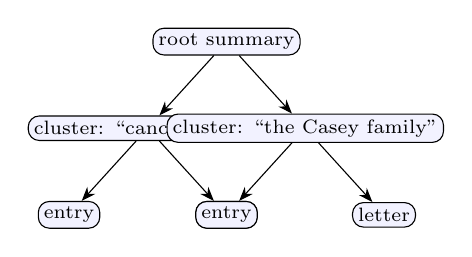
\begin{tikzpicture}[font=\scriptsize, level distance=11mm, sibling distance=20mm,
   every node/.style={draw, rounded corners, inner sep=2pt, fill=blue!5},
   edge from parent/.style={draw,-{Stealth[length=1.8mm]}}]
  \node {root summary}
    child {node {cluster: ``cancer favors''}
      child {node {entry}}
      child {node {entry}}}
    child {node {cluster: ``the Casey family''}
      child {node {entry}}
      child {node {letter}}};
\end{tikzpicture}
\end{center}

% =============================================================================
\section{How to run it, and the honest caveats}
% =============================================================================

\subsection*{Recommended settings}
\begin{itemize}[leftmargin=*]
  \item \textbf{Free smoke test:} \code{python -m lib.retrieval "your question"} --- prints the
        route, the grade, the hits with citations, and a \$0 cost ledger.
  \item \textbf{Pre-filter for free} with \code{where}, e.g.
        \code{where=\{"kind": "notebook\_entry"\}} or a callable year-predicate over the date string,
        to narrow the search before ranking.
  \item \textbf{Dial up quality} by opting into spend: \code{use\_rerank} (local free, cloud paid),
        \code{use\_multiquery} (RAG-Fusion), \code{auto\_apply\_route} (let the agent escalate).
\end{itemize}

\begin{caveatbox}[Caveats --- read before trusting a result or a toggle]
\begin{itemize}[leftmargin=*]
  \item \textbf{Dense needs an index.} \code{use\_dense=True} does nothing until that space's vector
        partition exists; \code{retrieve} quietly degrades to BM25-only by design --- you see lexical
        results, not an error.
  \item \textbf{The local reranker is not the named one.} fastembed packages
        \code{bge-reranker-base}, not the \code{bge-reranker-v2-m3} named in config; the local path
        substitutes the base model. Wire FlagEmbedding / sentence-transformers for the exact weights
        (the heavy torch dependency is deliberately not auto-installed).
  \item \textbf{Grading is a guardrail, not ground truth.} \code{grade\_context} returns a heuristic
        confidence, not a probability; tune the thresholds against a golden Q\&A set.
  \item \textbf{Contextual / ColPali / RAPTOR are documented, not yet coded here.} They are upstream
        or heavy and are deferred with TODOs --- this packet is explicit about wired-versus-planned.
  \item \textbf{Prices in \file{config.py} are placeholders.} Nothing is billed until a stage runs,
        and David has not said go. Confirm provider pricing before any billed sweep.
\end{itemize}
\end{caveatbox}

% =============================================================================
\section{Sources}
% =============================================================================

\begin{itemize}[leftmargin=*]
  \item Contextual Retrieval ($-67\%$ failures):
        \url{https://www.datacamp.com/tutorial/contextual-retrieval-anthropic};
        \url{https://www.freecodecamp.org/news/how-contextual-embeddings-and-hybrid-search-fix-retrieval-failures/}
  \item Advanced RAG, hybrid + RRF + rerank:
        \url{https://atlan.com/know/advanced-rag-techniques/};
        \url{https://machinelearningmastery.com/beyond-vector-search-5-next-gen-rag-retrieval-strategies/}
  \item RAPTOR: \url{https://ragflow.io/blog/long-context-rag-raptor};
        RAG vs GraphRAG eval: \url{https://arxiv.org/html/2502.11371v3}
  \item Multimodal / ColPali (late interaction):
        \url{https://weaviate.io/blog/late-interaction-overview};
        \url{https://huggingface.co/learn/cookbook/multimodal_rag_using_document_retrieval_and_reranker_and_vlms}
  \item Adaptive / router RAG ($-28\%$ cost, $+8\%$ accuracy):
        \url{https://arxiv.org/pdf/2604.03455};
        \url{https://www.llamaindex.ai/blog/rag-is-dead-long-live-agentic-retrieval}
  \item Self-RAG / CRAG (grade, reflect, abstain), RAG 2026 blueprint:
        \url{https://dev.to/suraj_khaitan_f893c243958/-rag-in-2026-a-practical-blueprint-for-retrieval-augmented-generation-16pp}
\end{itemize}

\noindent See \file{RESEARCH\_PLAN.md} Part~D for the full ranked frontier and the tiered roadmap
(Tier~0 = this module: contextual retrieval $+$ hybrid $+$ RRF $+$ rerank $+$ adaptive router $+$
cited generation $+$ evaluation).

\end{document}
